\documentclass[prb,11pt,twocolumn]{revtex4-1}

\usepackage{amsmath}
\usepackage{amssymb}
\usepackage{verbatim} 
\usepackage[draft]{graphicx} % need to fix images

% \graphicspath{{./2_2D_spatial_cross_correlation/data/}}
\graphicspath{{./2_2D_spatial_cross_correlation/docs/images/}}

\begin{document}

\title{Manuscript Title:\\with Forced Linebreak}% Force line breaks with \\
\date{\today}

\maketitle

\section{Background}
We want to find Wally, or in our case \textit{Rocketman} with a similar penchant for associating with dozens or more people at an interesting location, in this case: a maze.

Rocketman is shown in Figure\ref{fig:rocketman} and the maze in which Rocketman can be found is shown in Figure \ref{fig:maze}. 

\begin{figure}
    \includegraphics[]{rocketman.pdf}
    \caption{Rocketman!}
    \label{fig:rocketman}
\end{figure}

\begin{figure}
     \includegraphics[width=8cm]{maze.pdf}
     \caption{Rocketman can be found in this maze.}
     \label{fig:maze}
\end{figure}

My task is to find Rocketman in the Maze using the 2D cross correlation.

\section{Approach}
Figure~\ref{fig:maze} is $(1526\,\times\,2446)$ pixels for a total of 3,732,596 pixels and Figure~\ref{fig:rocketman} is $(111\,\times\,123)$ pixels for a total of 13,653 pixels. Using brute force (moving pixel by pixel) places an upper limit in the order of many millions; alternatively Rocketman fits $\approx300$ into the maze, and thus 'grid-searching' for Rocketman in grids the size of a $(111\,\times\,123)$ box and honing in could also require many operations in the order of minutes.

My approach is to first to take a non-transparent slice of Rocketman as shown in Figure~\ref{fig:rocketman_slice} say along row $j$ (see \texttt{solid\_row} in \texttt{get\_wally.py}), and choose one pixel $P_{(i,j)}$ from this slice (where $i,j\,\epsilon\,\mathbb{N}$, $0<i<111$ and $0<j<123$). From this slice I one pixel (\texttt{selected\_pixel}) with $P_{(i,j)}=(R,G,B,A)=(r_i,g_i,b_i,a_i)$, where $i\,\epsilon{(0,1,..,255)}$ and specifies the colour and transparency of $P_{(i,j)}$. 

\begin{figure}
     \includegraphics[width=8cm]{rocketman_slice.pdf}
     \caption{A ten pixel thick slice of Rocketman for illustrative purposes. I only take a one-pixel slice in my approach which would be difficult to see here.}
     \label{fig:rocketman_slice}
\end{figure}

In the maze $M$ (Figure~\ref{fig:maze}) I look for all instances of $P_{(i,j)}$ such that $M_{(k,l)}=P_{(i,j)}\,\forall{k,l}$ (where $k,l\,\epsilon\,\mathbb{N}$, $0<k<1526$ and $0<l<2446$) (see: \texttt{indices\_of\_selected\_pixel\_in\_template}). 

I look for all the $M_{(k,l)}$ to reduce my search area in the maze, to 13 points or less (so long as a black pixel isn't chosen). Figure~\ref{fig:maze-hist} is a histogram of all colours in the maze (arranged by hex number), each bar is the same colour it represents, and the height counts the number of times the pixel occurs in the the maze (Figure~\ref{fig:maze}). Here Figure~\ref{fig:maze-hist} is truncated at $y=5$ so less-frequent colours are easier to see, however the second-most common colour is white $(R,G,B,A)=(255,255,255,255)$ appearing 13 times, followed by a light green pixel $(R,G,B,A)=(199,255,142)$ which appears seven times. For comparison, black pixels $(R,G,B,A)=(0,0,0,255)$ are found 141 times in the maze.

\begin{figure}
     \includegraphics[width=8cm]{maze-colour-hist.pdf}
     \caption{A histogram of each RGB colour in used in the maze, each bar is coloured the pixel it counts.}
     \label{fig:maze-hist}
\end{figure}

I further reduce my search area by using a method inspired by the Boyer–Moore string-search algorithm: I look at the last pixels on either side of the Rocketman-slice $P_{(i-n,j)}$, $P_{(i+m,j)}$, and look for the same pixels, at the same location with respect to $M_{(k,l)}$. That is I expect $M_{(k-n,l)=P_{(i-n,j)}}$ and $M_{(k+m,l)=P_{(i+m,j)}}$ for one or more values of $(k,l)$ (see \texttt{right\_match} and \texttt{left\_match}).

To illustrate the above, a blue pixel in rocketman at $P_{(50,55)}$ with RGBA values $(R,G,B,A)=(156,255,255,255)$, are shown in the Figure~\ref{fig:maze-hist} (all other pixels are black for contrast). By starting my search around $M_{(k,l)}=P_{(50,55)}$ it saves me searching the whole grid for Rocketman.

\begin{figure}
     \includegraphics[width=8cm]{blue_pixels_in_maze.pdf}
     \caption{Given $P_{50,55}$ in Rocketman, I search for the same colour in the maze. This image shows the multiple locations in the maze where this type of blue is found (note all pixels a different colour to $P_{50,55}$ are coloured black for contrast).}
     \label{fig:maze-blue}
\end{figure}

From Figure~\ref{fig:maze-blue} there are roughly four possible search locations in the maze to start looking for Rocketman, I use the `end' pixels of the Rocketman slice to further narrow the search. Figure~\ref{fig:pixel-search} is a schematic of the process: the randomly selected pixel at $P_{(i,j)}$  (the blue pixel from the rocketman slice) sits in a row which ends in a red $P_{(i-n,j)}$ and blue pixel $P_{(i+m,j)}$. For each of the blue pixels in the maze at $M_{(k,l)}$ I look for red pixel at $M_{(k-n,l)}$ and a blue pixel at $M_{(k+m,l)}$. When these conditions are met my search location is narrowed further.

\begin{figure}
     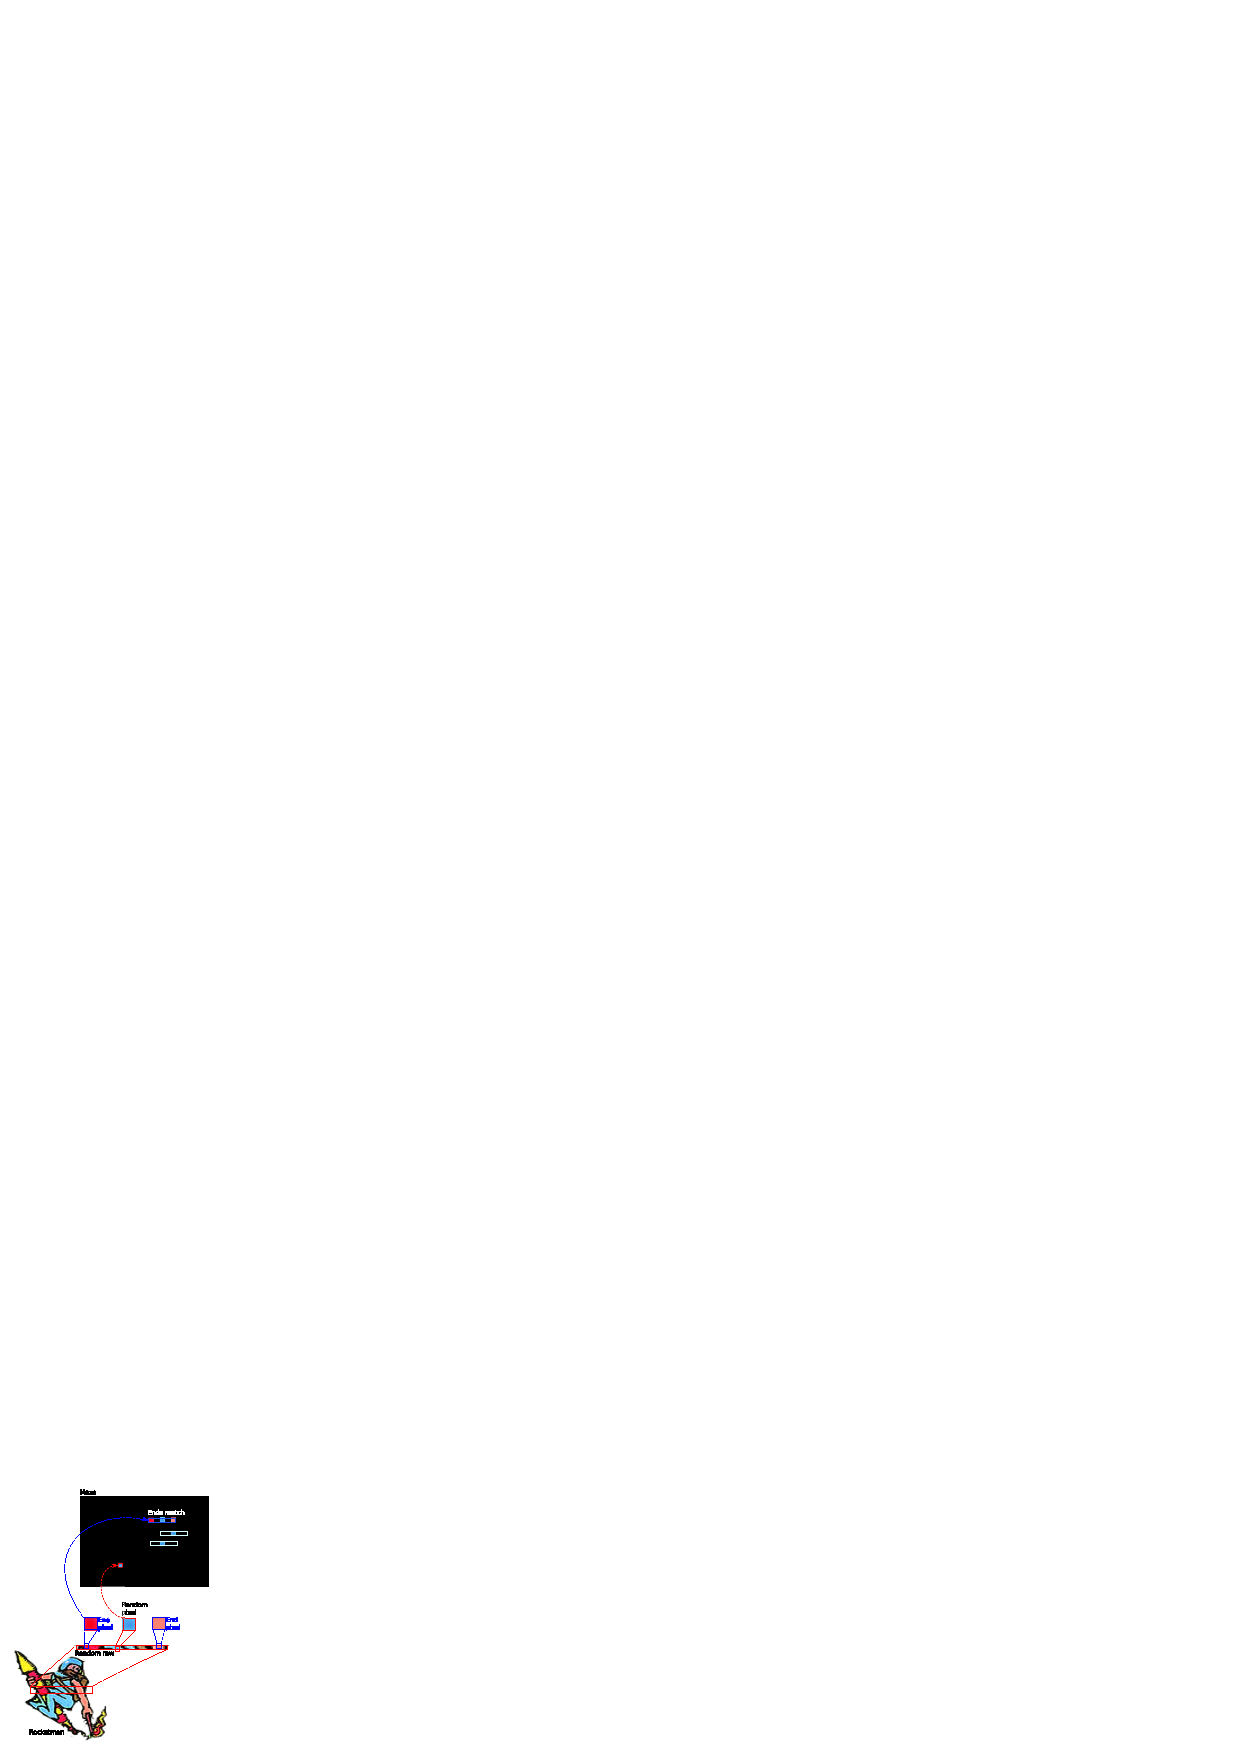
\includegraphics[width=8cm]{search_approach.pdf}
     \caption{A row is chosen from Rocketman (bottom), from which three pixels are chosen: two end pixels shown here in blue ($P_{(i-n,j)}$) and red ($P_{(i+m,j)}$) and a random pixel in between ($P_{(i,j)}$). The maze above illustrates after the blue pixel is found ($M_{(k,l)}=P_{(i,j)}$), I look for red pixel $-n$ away and blue pixel $+m$ away.}
     \label{fig:pixel-search}
\end{figure}

It's important to note that Rocketman is surrounded by pixels with some degree of transparency, this means choosing the "end" pixel in a row slice is not a matter of looking the first and last pixel, but the first and last solid pixel in the row. Figure~\ref{fig:pixel-pink} below colours all transparent pixels hot pink to highlight the point.

\begin{figure}
     \includegraphics[width=8cm]{rocketman_hotpink.pdf}
     \caption{Transparent pixels are coloured in hot-pink to highlight their}
     \label{fig:pixel-pink}
\end{figure}

With the search locations narrowed down the 2D cross correlation can be used to confirm the location of Rocketman.

The benefit of this approach is speed, and for the edgecase where there are more than one Rocketman in the maze. 

\section{Results}
Rocketman was found in under a second (usually around $0.4\,~\mathrm{sec}$) at position $\mathrm{(row,\,column)}=(651,\,981)$.

\texttt{get\_wally.py} will work for any image subset of the maze.

\section{Improvements}
My code is not built to handle rows where the image has transparent pixels in between two groups of solid pixels. This edge case could probably be worked out, however for this project I worked around this by selecting the a row with the longest row of solid pixels (see \texttt{max\_pixels}).

\end{document}